\documentclass{beamer}
\usetheme{Madrid}

\usepackage{multimedia}
\usepackage{algorithm}
\usepackage{algpseudocode}

\title{Master Thesis Presentation}
\subtitle{Optimal Transport in Linear Independent Component Analysis}
\author{Ashutosh Jha}
\institute{University of Tuebingen}
\date{October 2025}

\begin{document}

% Title frame
\begin{frame}
  \titlepage
\end{frame}

% Table of Contents
\begin{frame}{Outline}
  \tableofcontents
\end{frame}

\section{Introduction}

\begin{frame}{Introduction (1/3)}
  \begin{itemize}
    \item Linear Independent Component Analysis (ICA) seeks to recover a set of statistically independent components from their linear mixtures.
    \item Unlike Principal Component Analysis (PCA), which only ensures uncorrelated components, ICA imposes the stronger condition of full statistical independence.
    \item This stronger criterion allows ICA to disentangle latent variables that PCA cannot fully separate.
  \end{itemize}
\end{frame}

\begin{frame}{Introduction (2/3)}
  \begin{itemize}
    \item The approach builds upon intuition from the Central Limit Theorem: mixtures of independent random variables tend towards Gaussian distributions regardless of original distributions.
    \item Consequently, any mixture of independent \textbf{non-Gaussian} sources appears more Gaussian than the original sources themselves.
    \item After whitening the mixed signal to remove correlations, the problem reduces to finding a rotation on the unit sphere that maximizes non-Gaussianity.
  \end{itemize}
\end{frame}

\begin{frame}{Introduction (3/3)}
  \begin{itemize}
    \item The goal is to identify directions where projected data are least Gaussian, corresponding to candidate statistically independent components.
    \item To formalize this as an optimization problem, we measure Gaussianity using the Wasserstein-2 (W2) distance between the empirical distribution of projections and a Gaussian distribution.
    \item This distance comes from Optimal Transport theory, which quantifies the minimal “cost” of morphing one probability distribution into another.
  \end{itemize}
\end{frame}

\section{Independent Component Analysis Problem}

\begin{frame}{ICA Model}
The linear ICA model assumes that the observed signals are linear mixtures of statistically independent sources:
\[
\mathbf{X} = \mathbf{A} \mathbf{S}
\]
where
\[
\mathbf{X} = 
\begin{bmatrix}
x_1 \\
x_2 \\
\vdots \\
x_n
\end{bmatrix},
\quad
\mathbf{S} = 
\begin{bmatrix}
s_1 \\
s_2 \\
\vdots \\
s_n
\end{bmatrix},
\quad
\mathbf{A} = 
\begin{bmatrix}
a_{11} & a_{12} & \cdots & a_{1n} \\
a_{21} & a_{22} & \cdots & a_{2n} \\
\vdots & \vdots & \ddots & \vdots \\
a_{n1} & a_{n2} & \cdots & a_{nn}
\end{bmatrix}
\]

The sources \( s_i \) are assumed to be statistically independent, and at most one \( s_i \) can be Gaussian, since a mixture of Gaussian signals remains Gaussian and cannot be separated by ICA \cite{JuttenHerault1985}.
\end{frame}

\section{Mathematical Foundations ICA}

\begin{frame}{Centering}
  \begin{itemize}
    \item Observed mixtures: $\mathbf{X} \in \mathbb{R}^d$.
    \item Center before further processing: $\mathbb{E}[\mathbf{X}] = \mathbf{0}$.
    \item Covariance formula:
      \[
        \mathrm{Cov}(\mathbf{X}) = \mathbb{E}[\mathbf{X}\mathbf{X}^\top] - \mathbb{E}[\mathbf{X}]\mathbb{E}[\mathbf{X}]^\top
      \]
    \item If $\mathbb{E}[\mathbf{X}] = 0$ then
      \[
        \mathrm{Cov}(\mathbf{X}) = \mathbb{E}[\mathbf{X}\mathbf{X}^\top]
      \]
  \end{itemize}
\end{frame}


\begin{frame}{Whitening: Decorrelating with Eigenvalue Decomposition}
  \begin{itemize}
    \item Start with centered data $\mathbf{X} \in \mathbb{R}^d$.
    \item Compute the covariance matrix:
    \[
      \mathrm{Cov}(\mathbf{X}) = \mathbb{E}[\mathbf{X}\mathbf{X}^\top]
    \]
    \item Eigenvalue decomposition of covariance:
    \[
      \mathrm{Cov}(\mathbf{X}) = \mathbf{V}\mathbf{\Lambda}\mathbf{V}^\top
    \]
    where $\mathbf{U}$: eigenvectors, $\mathbf{\Lambda}$: diagonal matrix of eigenvalues.
    \item Apply decorrelation transform:
    \[
      \mathbf{W} = \mathbf{V}^\top
    \]
    \item $\mathbf{W}\mathbf{X}$ yields a diagonal covariance matrix with variance entries $\lambda_j$, but not necessarily unit variance.
  \end{itemize}
\end{frame}

\begin{frame}{Whitening: Scaling to Identity Covariance}
  \begin{itemize}
    \item To "whiten" data, rescale each decorrelated dimension to have unit variance.
    \item Whitening transformation:
    \[
      \mathbf{W} = \mathbf{\Lambda}^{-1/2} \mathbf{V}^\top
    \]
    Here, $\mathbf{\Lambda}^{-1/2}$ scales diagonal entries by $1/\sqrt{\lambda_j}$.
    \item Whitened data:
    \[
      \widetilde{\mathbf{X}} = \mathbf{W}\mathbf{X}
    \]
    \item Covariance after whitening:
    \[
      \mathrm{Cov}(\widetilde{\mathbf{X}}) = \mathbf{W}\mathrm{Cov}(\mathbf{X})\mathbf{W}^\top = \mathbf{I}_d
    \]
    \item Eigenvalue decomposition decorrelates data; scaling by $\mathbf{\Lambda}^{-1/2}$ gives unit variance.
  \end{itemize}
\end{frame}


\begin{frame}{Whitening and Scaling}
  \begin{itemize}
    \item Scaling the data so all dimensions have unit variance and are uncorrelated.
    \item Found (with ED/SVD) a linear $\mathbf{W}$ that gives $\widetilde{\mathbf{X}} = \mathbf{W}\mathbf{X}$ s.t.
      \[
         \mathrm{Cov}(\widetilde{\mathbf{X}}) = \mathbb{E}[\widetilde{\mathbf{X}} \widetilde{\mathbf{X}}^\top] = \mathbb{E}[\mathbf{W}\mathbf{X}\mathbf{X}^\top\mathbf{W}^\top]
         = \mathbf{W}\mathbb{E}[\mathbf{X}\mathbf{X}^\top]\mathbf{W}^\top
      \]

      \[
         \mathrm{Cov}(\widetilde{\mathbf{X}})
         = \mathbf{W}\mathrm{Cov}(\mathbf{X})\mathbf{W}^\top
      \]
    \item Diagonalized covariance:
      \[
        \mathrm{Cov}(\widetilde{\mathbf{X}}) = 
        \mathbf{W} \mathrm{Cov}(\mathbf{X}) \mathbf{W}^\top = \mathbf{D}
      \]
      but we choose scaling ($\mathbf{\Lambda}^{-1/2}$) such that $\mathbf{D} = \mathbf{I}_d$.
    \item \textbf{Why this scaling?}
      \begin{itemize}
        \item Ensures all dimensions are comparable.
        \item Reduces ICA problem to a rotation (orthogonal search, next slide).
      \end{itemize}
  \end{itemize}
\end{frame}

\begin{frame}{Unmixing}
  \begin{itemize}
    \item After whitening, seek a matrix $\mathbf{U}$ to "unmix" such that:
      \[
        \widetilde{\mathbf{Z}} = \mathbf{U} \widetilde{\mathbf{X}}
      \]
      where $\widetilde{\mathbf{Z}}$ is an estimated candidate vector for independent components.
    \item Covariance after unmixing:
      \[
        \mathrm{Cov}(\widetilde{\mathbf{Z}}) = \mathbf{U}\, \mathrm{Cov}(\widetilde{\mathbf{X}}) \, \mathbf{U}^\top = \mathbf{U} \mathbf{I}_d \mathbf{U}^\top = \mathbf{U}\mathbf{U}^\top
      \]
    \item When $\mathbf{U}$ is orthogonal ($\mathbf{U}\mathbf{U}^\top = \mathbf{I}_d$), recovered components are uncorrelated and ready for independence optimization.
    \item ICA then finds the rotation that makes elements of $\widetilde{\mathbf{Z}}$ as independent as possible.
  \end{itemize}
\end{frame}


\begin{frame}{Why PCA is not sufficient?}
\begin{enumerate}
  \item Make sample decorrelated and whitened, i.e. \( E[\mathbf{X}] = 0 \), \( E[\mathbf{X} \mathbf{X}^T] = \mathbf{I} \). At this point, any orientation is good enough for PCA, so it is not sufficient for ICA, when the data are non gaussian. For multivariate gaussian data decorrelation implies independence, so there is not much more for ICA to do.
  \item For ICA, find local optima of the function \( f(\mathbf{u}) = E[(\mathbf{u}^T \mathbf{X})^4] \) where \( \mathbf{u} \in S_n \) (unit sphere). Gradient descent can be used to find candidate components.
\end{enumerate}

\end{frame}


\section{Information Geometry and ICA}

\begin{frame}{Information Geometry Perspective on ICA}
  \begin{itemize}
    \item ICA aims to find a linear transform \(B\) such that \(Y = BX\) has maximally independent components.
    \item Standard decorrelation (whitening) gives uncorrelated axes, but not full independence unless data are Gaussian.
    \item Information geometry relates independence and non-Gaussianity: ICA projects distributions onto product and Gaussian manifolds to quantify both phenomena \cite{cardoso2022}.
  \end{itemize}
\end{frame}

\begin{frame}{Manifolds of Product and Gaussian Distributions}
  \begin{itemize}
    \item \(\mathcal{P}\): Product manifold -- distributions where all components are independent.
    \item \(\mathcal{G}\): Gaussian manifold -- all multivariate Gaussians (zero mean, fixed covariance).
    \item ICA seeks a projection of the empirical distribution onto \(\mathcal{P}\): the closest independent representation.
    \item After whitening, ICA operates on the intersection where covariance is identity and independence must be achieved via some optimization on rotated candidates.
  \end{itemize}
\end{frame}

\begin{frame}{KL Pythagorean Identity on Product Manifold}
  \begin{itemize}
    \item For any random vector \(Y\) with density \(P_Y\), mutual information is denoted by \(\mathscr{L}(Y)\):
      \[
        \mathscr{I}(Y) = D_{\mathrm{KL}}(P_Y \,\Vert \, \prod_{i} P_{Y_i})
      \]
    \item More generally, for any product candidate \(Q = \prod_{i} q_i\):
      \begin{align*}
      D_{\mathrm{KL}}\left(P_Y \Vert Q\right)
      &= D_{\mathrm{KL}}\left(P_Y \Vert \prod_{i} P_{Y_i}\right) + D_{\mathrm{KL}}\left(\prod_{i} P_{Y_i} \Vert \prod_{i} q_{i}\right) \\
      &= D_{\mathrm{KL}}\left(P_Y \Vert \prod_{i} P_{Y_i}\right) + \sum_{i} D_{\mathrm{KL}}\left(P_{Y_i} \Vert q_i\right) \\
      &= \mathscr{I}(Y) + \sum_{i} D_{\mathrm{KL}}\left(P_{Y_i} \Vert q_i\right)
    \end{align*}
    \item Minimizing KL to a product model first projects onto marginals; the leftover is mutual information.
  \end{itemize}
\end{frame}

\begin{frame}{KL Pythagorean Identity on Gaussian Manifold}
  $$
      D_{\mathrm{KL}}\big(P_Y \Vert N(\Sigma)\big) = D_{\mathrm{KL}}\big(P_Y \Vert N(\operatorname{Cov} Y)\big) + D_{\mathrm{KL}}\big(N(\operatorname{Cov} Y) \Vert N(\Sigma)\big)
    $$
  \begin{itemize}
    \item $N(\Sigma)$ denotes the multivariate Gaussian distribution with covariance $\Sigma$ and zero mean.
    \item $N(\operatorname{Cov} Y)$ is the Gaussian with the empirical mean and covariance matrix of $Y$.
    \item This formula expresses that KL divergence from $P_Y$ to any Gaussian splits into the divergence to the best Gaussian fit (same covariance as $Y$) and the divergence between two Gaussian distributions (with covariances $\operatorname{Cov} Y$ and $\Sigma$).
  \end{itemize}
\end{frame}

\begin{frame}{Combining Pythagorean Theorems}
  
  Let us combine the Pythagorean theorem for independence with the one for Gaussianity, interpreting ICA as successive geometric approximations:
  \begin{itemize}
    \item For an $N$-vector with complicated joint distribution $P_Y$, two simplifying approximations are:
      \begin{itemize}
        \item \textbf{Gaussian}: $P^G_Y \equiv \mathcal{N}(\operatorname{Cov}Y)$  -- best Gaussian fit (project onto $\mathcal{G}$).
        \item \textbf{Product}: $P^P_Y \equiv \prod_i P_{Y_i}$ -- distribution with independent marginals (project onto $\mathcal{P}$).
      \end{itemize}
    \item Applying both approximations yields $P^{PG}_Y \equiv \mathcal{N}(\operatorname{diag\,Cov}Y)$, a Gaussian with independent marginals matching those of $Y$.
    \item These yield two triangles through distribution space: $[P_Y \to P^G_Y \to P^{PG}_Y]$ and $[P_Y \to P^P_Y \to P^{PG}_Y]$, sharing the hypotenuse $[P_Y \to P^{PG}_Y]$.
  \end{itemize}
\end{frame}

\begin{frame}{Information Geometry in ICA}
  \begin{center}
    
\includegraphics[width=0.7\textwidth]{pythagorean_ig_ica.png}
  \end{center}
\end{frame}

\begin{frame}{Combining Pythagorean Theorems}
    The KL divergence to the product-Gaussian approximation admits two complementary decompositions:
    \[
      D\big[P_Y \Vert P^{PG}_Y\big] = D\big[P_Y \Vert P^P_Y\big] + D\big[P^P_Y \Vert P^{PG}_Y\big] = D\big[P_Y \Vert P^G_Y\big] + D\big[P^G_Y \Vert P^{PG}_Y\big]
    \]

  \begin{itemize}
    \item \textbf{Mutual Information:} $I(Y) = D[P_Y \Vert P^P_Y]$  
    \item \textbf{Non-Gaussianity:} $G(Y) = D[P_Y \Vert P^G_Y]$
    \item \textbf{Correlation Scalar:}
      \[
      C(Y) = D\big[P^G_Y \Vert P^{PG}_Y\big] = D[\mathcal{N}(\operatorname{Cov}Y) \Vert \mathcal{N}(\operatorname{diag\,Cov}Y)]
      \]
      Measures how far the $\operatorname{Cov}Y$ matrix is from just it's diagonal part and appears as the natural scalar measure of the correlation between entries of $Y$.
  \end{itemize}
\end{frame}

\begin{frame}{Non-Gaussianity, correlation and independence}
  \begin{itemize}
    \item Define non-Gaussianity of \(Y\):
      \[
        G(Y) = D_{\mathrm{KL}}(P_Y \,\Vert\, N(\operatorname{Cov}(Y)))
      \]
    \item Cardoso's pythagorean theorem relates independence, correlation, and non-Gaussianity:
      \[
        \mathscr{L}(Y) + \sum_{i} G(Y_i) = C(Y) + G(Y)
      \]
    \item Where
      \begin{itemize}
        \item \(C(Y) = D_{\mathrm{KL}}(N(\operatorname{Cov}(Y)) \,\Vert\, N(\operatorname{diag\,Cov}(Y)))\) measures how correlated the Gaussian approximation of Y and decorrelated? Y is.
        \item \(G(Y)\) is joint non-Gaussianity; \(G(Y_i)\) is marginal non-Gaussianity.
      \end{itemize}
  \end{itemize}
\end{frame}

\begin{frame}{Invariant KL Divergence of Gaussian Projection}
    If $Y$ undergoes an invertible linear transformation, then its Gaussian projection $N(\operatorname{Cov}Y)$ undergoes the same transformation.
    The Kullback-Leibler divergence to the Gaussian projection is invariant:
    \[
      D_{\mathrm{KL}}\big(P_Y \,\Vert\, N(\operatorname{Cov}Y)\big)
      = D_{\mathrm{KL}}\big(P_{A^{-1}Y} \,\Vert\, N(A^{-1} \operatorname{Cov}Y (A^{-1})^\top)\big)
    \]
    
    That is, $G(Y)$ does not change under invertible linear transformations.
\end{frame}


\begin{frame}{Whitening Reduces ICA to Maximizing Non-Gaussianity}
  \begin{itemize}
    \item After whitening, \(\operatorname{Cov}(Y) = I\), so \(C(Y) = 0\): Pythagorean identity reduces to
      \[
        \mathscr{L}(Y) = 0 - \sum_{i} G(Y_i) + \text{const}
      \]
    \item ICA in whitened space therefore reduces to maximizing non-Gaussianity of the marginals, subject to orthogonality constraints.
    \item Contrast functions (kurtosis, negentropy, Wasserstein distances) measure this non-Gaussianity and solve ICA.
    \item Thus, Centering and whitening constrain data to the space where independence can be achieved solely by maximizing non-Gaussianity \cite{cardoso2022}.
  \end{itemize}
\end{frame}



\section{Motivations from the Central Limit Theorem}

%-------------------------------------------------------------
\begin{frame}{Motivations from Central Limit Theorem}
\begin{itemize}
    \item Let \( X_1, X_2, \ldots, X_n \) be independent and identically distributed (i.i.d.) random variables drawn from a non-Gaussian distribution with mean \( \mu \) and variance \( \sigma^2 \).
    \item Define the sample mean as
    \[
        \bar{X}_n = \frac{1}{n} \sum_{i=1}^{n} X_i
    \]
    \item The CLT states that as \( n \to \infty \), the distribution of
    \[
        \sqrt{n} \left(\bar{X}_n - \mu \right) 
        \xrightarrow[]{\,d\,} 
        Z \sim \mathcal{N}(0, \sigma^2)
    \]
    where the arrow \(\xrightarrow[]{d}\) denotes convergence in distribution.
\end{itemize}
\end{frame}


%-------------------------------------------------------------
\begin{frame}{Weighted Sum Interpretation of CLT}
\begin{itemize}
    \item The sample mean can be seen as a weighted sum:
    \[
        \bar{X}_n = \sum_{i=1}^{n} \frac{1}{n} X_i
    \]
    where all weights \( \frac{1}{n} \) are equal.
    \item If viewed as an expectation, this weighted sum is
    \[
        \mathbb{E}[X] = \sum_{i=1}^{n} w_i X_i, \quad \text{where} \quad w_i = \frac{1}{n}, \quad \sum_{i=1}^n w_i = 1.
    \]
    \item \textbf{Conclusion:} Any weighted mixture of non-Gaussian sources tends to be closer to a Gaussian distribution than the original sources themselves.
\end{itemize}
\end{frame}


\begin{frame}{Why Independent Components Cannot be Gaussian}
\begin{itemize}
    \item The fundamental assumption in Independent Component Analysis (ICA) is that the independent components must be non-Gaussian for the model to be identifiable and ICA to work.
    \item Gaussian components cannot be separated since any linear combination of Gaussian variables is also Gaussian. This means the mixing matrix cannot be uniquely estimated.
    \item For Gaussian Multivariate distributions decorrelation implies independence, so after PCA, decorrelation, there is not much more ICA can achieve.
    \item Motivation from the CLT: weighted sums of independent non-Gaussian variables tend toward Gaussianity, so we seek sources that are maximally non-Gaussian.\cite{hyvarinen2001independent}.
\end{itemize}
\end{frame}

\section{Optimal Transport}

%-------------------------------------------------------------
\begin{frame}{Introduction to Optimal Transport}
\begin{itemize}
    \item Optimal Transport (OT) is about moving "mass" in the most efficient way, akin to how one might move sand with minimal effort.
    \item The earth mover distance (EMD) quantifies this cost, measuring how much "work" it takes to transform one distribution into another.
    \item The problem was first formulated by Gaspard Monge in 1781, conceptualizing the minimal cost of moving soil \cite{monge1781}.
\end{itemize}
\end{frame}

%-------------------------------------------------------------
\begin{frame}{Optimal Transport for Probability Distributions}
\begin{itemize}
    \item The core idea is to measure distances between probability measures using the cost of transporting one distribution into another.
    \item This led to metrics such as the Wasserstein distance, which quantify meaningful differences between distributions.
    \item The Kantorovich relaxation generalized Monge's formulation using transport plans, allowing greater mathematical and computational tractability \cite{kantorovich1942, villani2003, villani2006}.
\end{itemize}
\end{frame}

\begin{frame}{Introducing Distance \(W_1\)}
\begin{itemize}
    \item \(W_1\) distance (Earth Mover's Distance) measures the minimal total "effort" to move one distribution into another.
    \item For one-dimensional distributions with CDFs \(F\) and \(G\), it can be written as:
    \[
        W_1(\mu, \nu) = \int_{-\infty}^\infty |F(x) - G(x)| \, dx
    \]
    \item Intuitively, \(W_1\) sums the absolute vertical differences between the cumulative distribution functions.
\end{itemize}
\end{frame}

\begin{frame}{Introducing Distance \(W_2\) and Comparison}
\begin{itemize}
    \item \(W_2\) distance uses squared differences and is given by:
    \[
        W_2(\mu, \nu) = \left( \int_0^1 |F^{-1}(t) - G^{-1}(t)|^2 \, dt \right)^{1/2}
    \]
    where \(F^{-1}, G^{-1}\) are the quantile functions (inverse CDFs).
    \item \(W_2\) is more sensitive to differences in spread (variance) and central location (mean).
    \item When comparing distributions with \(\mathcal{N}(0,1)\), \(W_2\) better captures deviations than \(W_1\), making it more reliable for Gaussianity measures.
    \item \(W_1\) can be more robust to outliers but might underestimate such deviations.
\end{itemize}
\end{frame}

% ----------------------------------------------------------------------
% Proof Section: Motivations for using W2 in ICA
% ----------------------------------------------------------------------

\section{Theoretical Motivation: W2 Upper Bound}

\begin{frame}{Motivation: Bounding Mixture Non-Gaussianity}
  \begin{itemize}
    \item \textbf{Goal:} We want to justify why maximizing $W_2$ recovers independent sources.
    \item \textbf{Claim:} The non-Gaussianity of a mixture $w \cdot Z$ is upper bounded by the weighted sum of the non-Gaussianity of its independent parts.
    \item 
      \[
        W_2^2(w \cdot Z, \mathcal{N}) \le \sum_{i=1}^{d} w_i^2 W_2^2(Z_i, \mathcal{N})
      \]
    \item \textbf{Interpretation?:} By the Central Limit Theorem, mixtures are "more Gaussian" (have lower $W_2$ distance to $\mathcal{N}$) than the sources. Maximizing the LHS forces the weight vector $w$ to align with a single source $Z_i$.
  \end{itemize}
\end{frame}

\begin{frame}{Proof Construction: The Common Source}
  To prove the bound, we construct a specific coupling using a common source of randomness.
  \begin{itemize}
    \item Let $\mathbf{N} = (N_1, \dots, N_d)$ be a vector of $d$ independent Standard Normal variables.
    \item Let $T_i$ be the Optimal Transport map such that $(T_i)_{\#} \mathcal{N} = Z_i$.
    \item \textbf{Constructing the Mixture Variable $X$:}
      \[
        X = \sum_{i=1}^d w_i T_i(N_i)
      \]
      Since $T_i(N_i) \sim Z_i$, it follows that $X \sim w \cdot Z$.
    \item \textbf{Constructing the Gaussian Target $Y$:}
      Using the \textit{same} noise vector $\mathbf{N}$:
      \[
        Y = \sum_{i=1}^d w_i N_i
      \]
      Since $\sum w_i^2 = 1$, it follows that $Y \sim \mathcal{N}(0,1)$.
  \end{itemize}
\end{frame}

\begin{frame}{Proof Step: The Coupling Inequality}
  \begin{itemize}
    \item The pair $(X, Y)$ creates a valid joint distribution (coupling) $\pi_{X,Y}^{\mathbf{N}}$.
    \item \textbf{Definition of Wasserstein-2:} The infimum of cost over \textit{all possible} couplings.
      \[
        W_2^2(w \cdot Z, \mathcal{N}) = \inf_{\pi} \mathbb{E}_{\pi}[|x - y|^2]
      \]
    \item \textbf{The Inequality:} Since the infimum is the cost of the \textit{best} plan, it must be less than or equal to the cost of \textit{our specific} plan.
      \[
        \underbrace{W_2^2(w \cdot Z, \mathcal{N})}_{\text{Cost of Optimal Plan}} \le \underbrace{\mathbb{E}[|X - Y|^2]}_{\text{Cost of our constructed plan}}
      \]
  \end{itemize}
\end{frame}

\begin{frame}{Proof Step: Expanding the Square}
  Let us expand the expected squared difference $\mathbb{E}[|X - Y|^2]$:
  \begin{align*}
    |X - Y|^2 &= \left| \sum_{i=1}^d w_i T_i(N_i) - \sum_{i=1}^d w_i N_i \right|^2 \\
              &= \left( \sum_{i=1}^d w_i (T_i(N_i) - N_i) \right)^2
  \end{align*}
  Squaring the sum yields diagonal terms ($i=j$) and cross terms ($i \neq j$):
  \[
    = \sum_{i=1}^d w_i^2 (T_i(N_i) - N_i)^2 + \sum_{i \neq j} w_i w_j (T_i(N_i) - N_i)(T_j(N_j) - N_j)
  \]
\end{frame}

\begin{frame}{Proof Conclusion: Vanishing Cross Terms}
  Taking the expectation $\mathbb{E}$:
  \begin{itemize}
    \item \textbf{Cross Terms ($i \neq j$):} vanish due to independence and zero mean.
      \[
        \mathbb{E}[\text{Cross}] \propto \mathbb{E}[T_i(N_i) - N_i] \cdot \mathbb{E}[T_j(N_j) - N_j] = 0 \cdot 0 = 0
      \]
    \item \textbf{Diagonal Terms:}
      \[
        \mathbb{E}[|X - Y|^2] = \sum_{i=1}^d w_i^2 \mathbb{E}[ |T_i(N_i) - N_i|^2 ]
      \]
    \item Recall that $\mathbb{E}[ |T_i(N_i) - N_i|^2 ]$ is exactly $W_2^2(Z_i, \mathcal{N})$.
    \item \textbf{Result:}
      \[
        W_2^2(w \cdot Z, \mathcal{N}) \le \sum_{i=1}^d w_i^2 W_2^2(Z_i, \mathcal{N})
      \]
      This convexity adjacent property confirms that mixtures reduce the Wasserstein distance to Gaussianity.
  \end{itemize}
\end{frame}

% ----------------------------------------------------------------------
%  Proof of Equality vs Strict Inequality
% ----------------------------------------------------------------------

\section{Proof of Strict Inequality}

\begin{frame}{Condition for Equality (1D Case)}
  \textbf{Brenier's Theorem and Comonotonicity:}
  \begin{itemize}
    \item We compare two scalar variables, $X$ and $Y$, constructed from the random vector $\mathbf{N} \in \mathbb{R}^d$.
    \item In the 1D case, the Wasserstein-2 distance satisfies $W_2^2(X, Y) = \mathbb{E}[|X-Y|^2]$ \textbf{if and only if} $X$ and $Y$ are \textbf{comonotonic}.
    \item This means there exists a strictly increasing function $f$ such that $X = f(Y)$.
    \item \textbf{Implication:} For this to hold, the gradients of $X$ and $Y$ with respect to the source noise $\mathbf{N}$ must be parallel at every point $\mathbf{N}$:
    \[ \nabla X(\mathbf{N}) = \lambda(\mathbf{N}) \nabla Y(\mathbf{N}) \]
    \textit{Note: The scaling factor $\lambda(\mathbf{N})$ is a scalar function of $\mathbf{N}$, not necessarily a constant.}
  \end{itemize}
\end{frame}

\begin{frame}{Definitions and Regularity}
  \textbf{Assumption (Regularity):}
  We assume the source distributions possess smooth, strictly positive densities. This guarantees that the optimal transport maps $T_i$ are \textbf{differentiable} functions (Luis Caffarelli regularity).

  \vspace{0.2cm}
  \textbf{Definitions:}
  \begin{itemize}
    \item Noise Vector: $\mathbf{N} = [N_1, N_2, \dots, N_d]^\top$
    \item Projection Vector: $\mathbf{w} = [w_1, w_2, \dots, w_d]^\top$
  \end{itemize}
  
  \textbf{1. The Gaussian Target Gradient:}
  \[ Y(\mathbf{N}) = \sum w_i N_i \implies \frac{\partial Y}{\partial N_k} = w_k \]
  \[ \implies \nabla Y = \mathbf{w} \]
\end{frame}

\begin{frame}{Computing the Mixture Gradient}
  \textbf{2. The Source Mixture Gradient:}
  \[ X(\mathbf{N}) = \sum_{i=1}^d w_i T_i(N_i) \]
  
  Applying the chain rule element-wise:
  \[ \frac{\partial X}{\partial N_k} = \frac{\partial}{\partial N_k} (w_k T_k(N_k)) = w_k T'_k(N_k) \]
  
  Writing as a vector:
  \[ \nabla X = \begin{bmatrix} w_1 T'_1(N_1) \\ w_2 T'_2(N_2) \\ \vdots \\ w_d T'_d(N_d) \end{bmatrix} \]
  
  \textbf{The Equality Condition:}
  We require $\nabla X = \lambda(\mathbf{N}) \mathbf{w}$.
\end{frame}

\begin{frame}{Applying the Product Rule}
  To test if $\nabla X = \lambda(\mathbf{N}) \mathbf{w}$ can hold for non-linear maps, we differentiate both sides with respect to $\mathbf{N}$ (computing the Hessian).
  
  \begin{itemize}
    \item \textbf{LHS (Hessian of $X$):}
      Since $X$ is a sum of independent terms $w_i T_i(N_i)$, cross-derivatives are zero. The Hessian is \textbf{Diagonal}.
      \[ \mathbf{H}_X = \text{diag}\left( w_1 T''_1(N_1), \dots, w_d T''_d(N_d) \right) \]

    \item \textbf{RHS (Product Rule):}
      We differentiate the product of scalar $\lambda(\mathbf{N})$ and constant vector $\mathbf{w}$.
      \[ \frac{\partial}{\partial \mathbf{N}} \left( \lambda(\mathbf{N}) \mathbf{w} \right) = \mathbf{w} (\nabla \lambda)^\top \]
      This results in a \textbf{Rank-1 Matrix} (outer product) where entry $(i,j)$ is $w_i \frac{\partial \lambda}{\partial N_j}$.
  \end{itemize}
\end{frame}

\begin{frame}{The Contradiction and Conclusion}
  We equate the LHS (Diagonal) and RHS (Rank-1):
  \[ \text{Diagonal Matrix} = \mathbf{w} (\nabla \lambda)^\top \]
  
  \textbf{Analysis:}
  \begin{itemize}
    \item The off-diagonal entries ($i \neq j$) of the LHS are exactly 0.
    \item Thus, the RHS off-diagonals must be 0: $w_i \frac{\partial \lambda}{\partial N_j} = 0$.
    \item Since weights $w_i \neq 0$ (for a mixture), we must have $\frac{\partial \lambda}{\partial N_j} = 0$ for all $j$.
    \item This implies $\nabla \lambda = \mathbf{0}$, so $\lambda$ is a \textbf{constant}.
  \end{itemize}
  
  \textbf{Final Result:}
  If $\lambda$ is constant, then $T'_i(N_i) = \lambda$ implies $T_i$ must be linear.
  \begin{itemize}
    \item Linear maps only exist for Gaussian sources.
    \item For non-Gaussian sources, this contradiction proves \textbf{Strict Inequality}.
  \end{itemize}
\end{frame}

% ----------------------------------------------------------------------
% Empirical Comparison W1 vs W2
% ----------------------------------------------------------------------

\section{Empirical Comparison: W1 vs W2}

\begin{frame}{Empirical Comparison: Experimental Setup}
  \begin{itemize}
    \item To select the optimal contrast function, we empirically compared the optimization landscape of $W_1$ (Mean Absolute Error) versus squared $W_2$ (Mean Squared Error).
    \item \textbf{Setup:}
      \begin{itemize}
        \item Synthetic data generated from Student-t distributions.
        \item We varied the degrees of freedom ($\nu$) to control "non-Gaussianity":
        \begin{itemize}
            \item $\nu=2$: Heavy tails (Strong non-Gaussian signal).
            \item $\nu=10$: Approaching Normal (Weak non-Gaussian signal).
        \end{itemize}
        \item We plotted the distance metric over the rotation angle $\theta$ relative to the first Principal Component.
      \end{itemize}
  \end{itemize}
\end{frame}

\begin{frame}{Case 1: Strong Non-Gaussianity ($\nu=2$)}
  \begin{columns}
    \begin{column}{0.6\textwidth}
      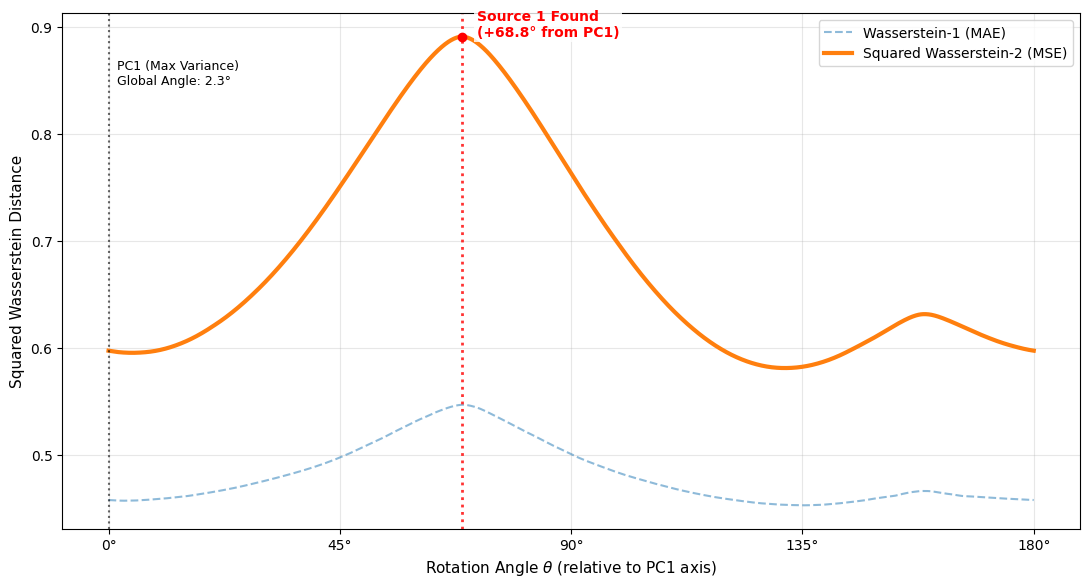
\includegraphics[width=\textwidth]{student_t_df2_strong.png} % Replace with image_9f1e5b.png
    \end{column}
    \begin{column}{0.4\textwidth}
      \textbf{Observation:}
      \begin{itemize}
        \item Both $W_1$ and $W_2$ successfully identify the source (peaks align).
        \item $W_2$ (orange) exhibits a significantly sharper peak and higher curvature around the optimum.
        \item This suggests $W_2$ provides stronger gradients for optimization when the signal is distinct.
      \end{itemize}
    \end{column}
  \end{columns}
\end{frame}

\begin{frame}{Case 2: Medium Non-Gaussianity ($\nu=4$)}
  \begin{columns}
    \begin{column}{0.6\textwidth}
      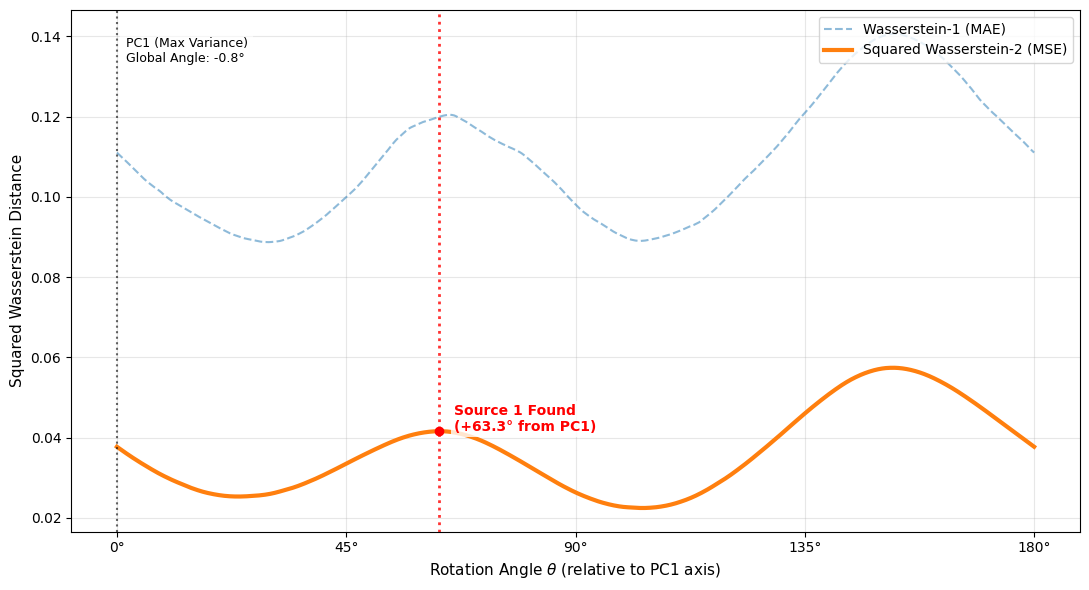
\includegraphics[width=\textwidth]{student_t_df4_mid.png} % Replace with image_9f1b39.png
    \end{column}
    \begin{column}{0.4\textwidth}
      \textbf{Observation:}
      \begin{itemize}
        \item As tails become lighter, the signal weakens.
        \item $W_2$ maintains a smooth, convex-like profile around the optimum.
        \item $W_1$ begins to show irregularities in the landscape, though the global maximum is still recoverable.
      \end{itemize}
    \end{column}
  \end{columns}
\end{frame}

\begin{frame}{Case 3: Weak Non-Gaussianity ($\nu=10$)}
  \begin{columns}
    \begin{column}{0.6\textwidth}
      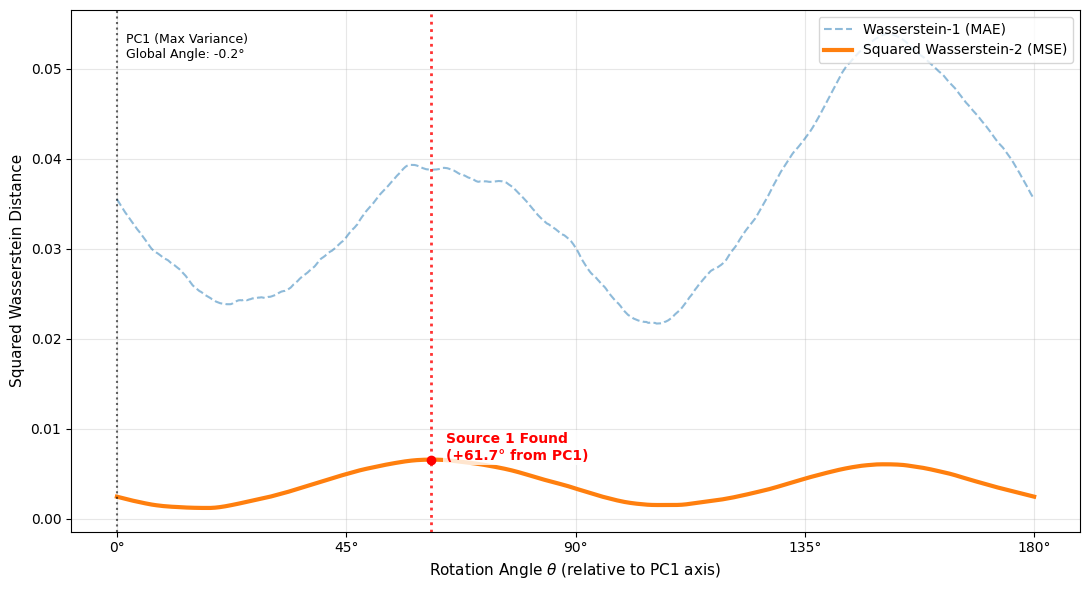
\includegraphics[width=\textwidth]{student_t_df10_weak.png} % Replace with image_9f17ed.png
    \end{column}
    \begin{column}{0.4\textwidth}
      \textbf{Crucial Difference:}
      \begin{itemize}
        \item The signal is now very close to Gaussian noise.
        \item \textbf{$W_1$ (blue dashed):} Becomes jagged and noisy. This "rough" landscape traps gradient-based solvers in spurious local optima.
        \item \textbf{$W_2$ (orange):} Remains smooth and unimodal.
        \item \textbf{Conclusion:} $W_2$ is slightly robust for weak signals, enabling recovery where $W_1$ fails.
      \end{itemize}
    \end{column}
  \end{columns}
\end{frame}




\section{Core Idea}

\begin{frame}{Core Idea: Optimization Problem with W2}
\begin{itemize}
    \item Traditional ICA formulations optimize kurtosis or negentropy contrast functions.
    \item Our approach formulates ICA as finding the rotation \(\mathbf{u} \in S_n\) that maximizes the W2 distance \((W_2)\) from the standard Gaussian \(\mathcal{N}(0,1)\):
    \[
        \hat{\mathbf{u}} = \arg\max_{\mathbf{u} \in S_n} W_2\big(\mathbb{P}_{\mathbf{u}^\top \mathbf{X}}, \mathcal{N}(0,1)\big)
    \]
    \item This perspective leverages the optimal transport metric's ability to capture deviations from Gaussianity in a geometrically meaningful way.
\end{itemize}
\end{frame}


\begin{frame}{Core Idea: Algorithm}
\begin{algorithm}[H]
\caption{ICA with W2 Distance Optimization}
\begin{algorithmic}[1]
\State Obtain observed mixture data \(\mathbf{X}\)
\State Perform whitening/decorrelation on \(\mathbf{X}\)
\State Initialize empty set of recovered components \(\mathcal{U} = \emptyset\)
\While{number of components not found}
    \State Find local optimum (Gradient Descent) \(\mathbf{u}^* \in S_n\) maximizing
    \[
        W_2\left(\mathbb{P}_{\mathbf{u}^\top \mathbf{X}}, \mathcal{N}(0,1)\right)
    \]
    \State Store candidate: \(\mathcal{U} \leftarrow \mathcal{U} \cup \{\mathbf{u}^*\}\)
    \State Restrict search space by enforcing orthogonality:
    \[
        \mathbf{u} \perp \mathrm{span}(\mathcal{U})
    \]
\EndWhile
\State \textbf{return} \(\mathcal{U}\) as estimated independent components
\end{algorithmic}
\end{algorithm}
\end{frame}





\section{Bibliography}

\begin{frame}[allowframebreaks]{References}
\bibliographystyle{alpha}
\bibliography{references.bib} % Your .bib file name here
\end{frame}


\end{document}
